\chapter{Manual examination of all DNMs in a single \textit{P. falciparum} sample}
\label{ch:pfscreenshots}

\section{Introduction}

To establish the veracity of our calls in the \textit{P. falciparum} crosses, we manually examined all events in a single sample, the 3D7xHB3 progeny PG0063-C.  This appendix presents several screenshots from IGV and our custom graph viewing software used to establish the visual veracity of the calls.  The calls depicted are taken from Table \ref{tbl:callsPG0063C}.

\section{Screenshots}

\begin{sidewaysfigure}[h!]
  \centering
    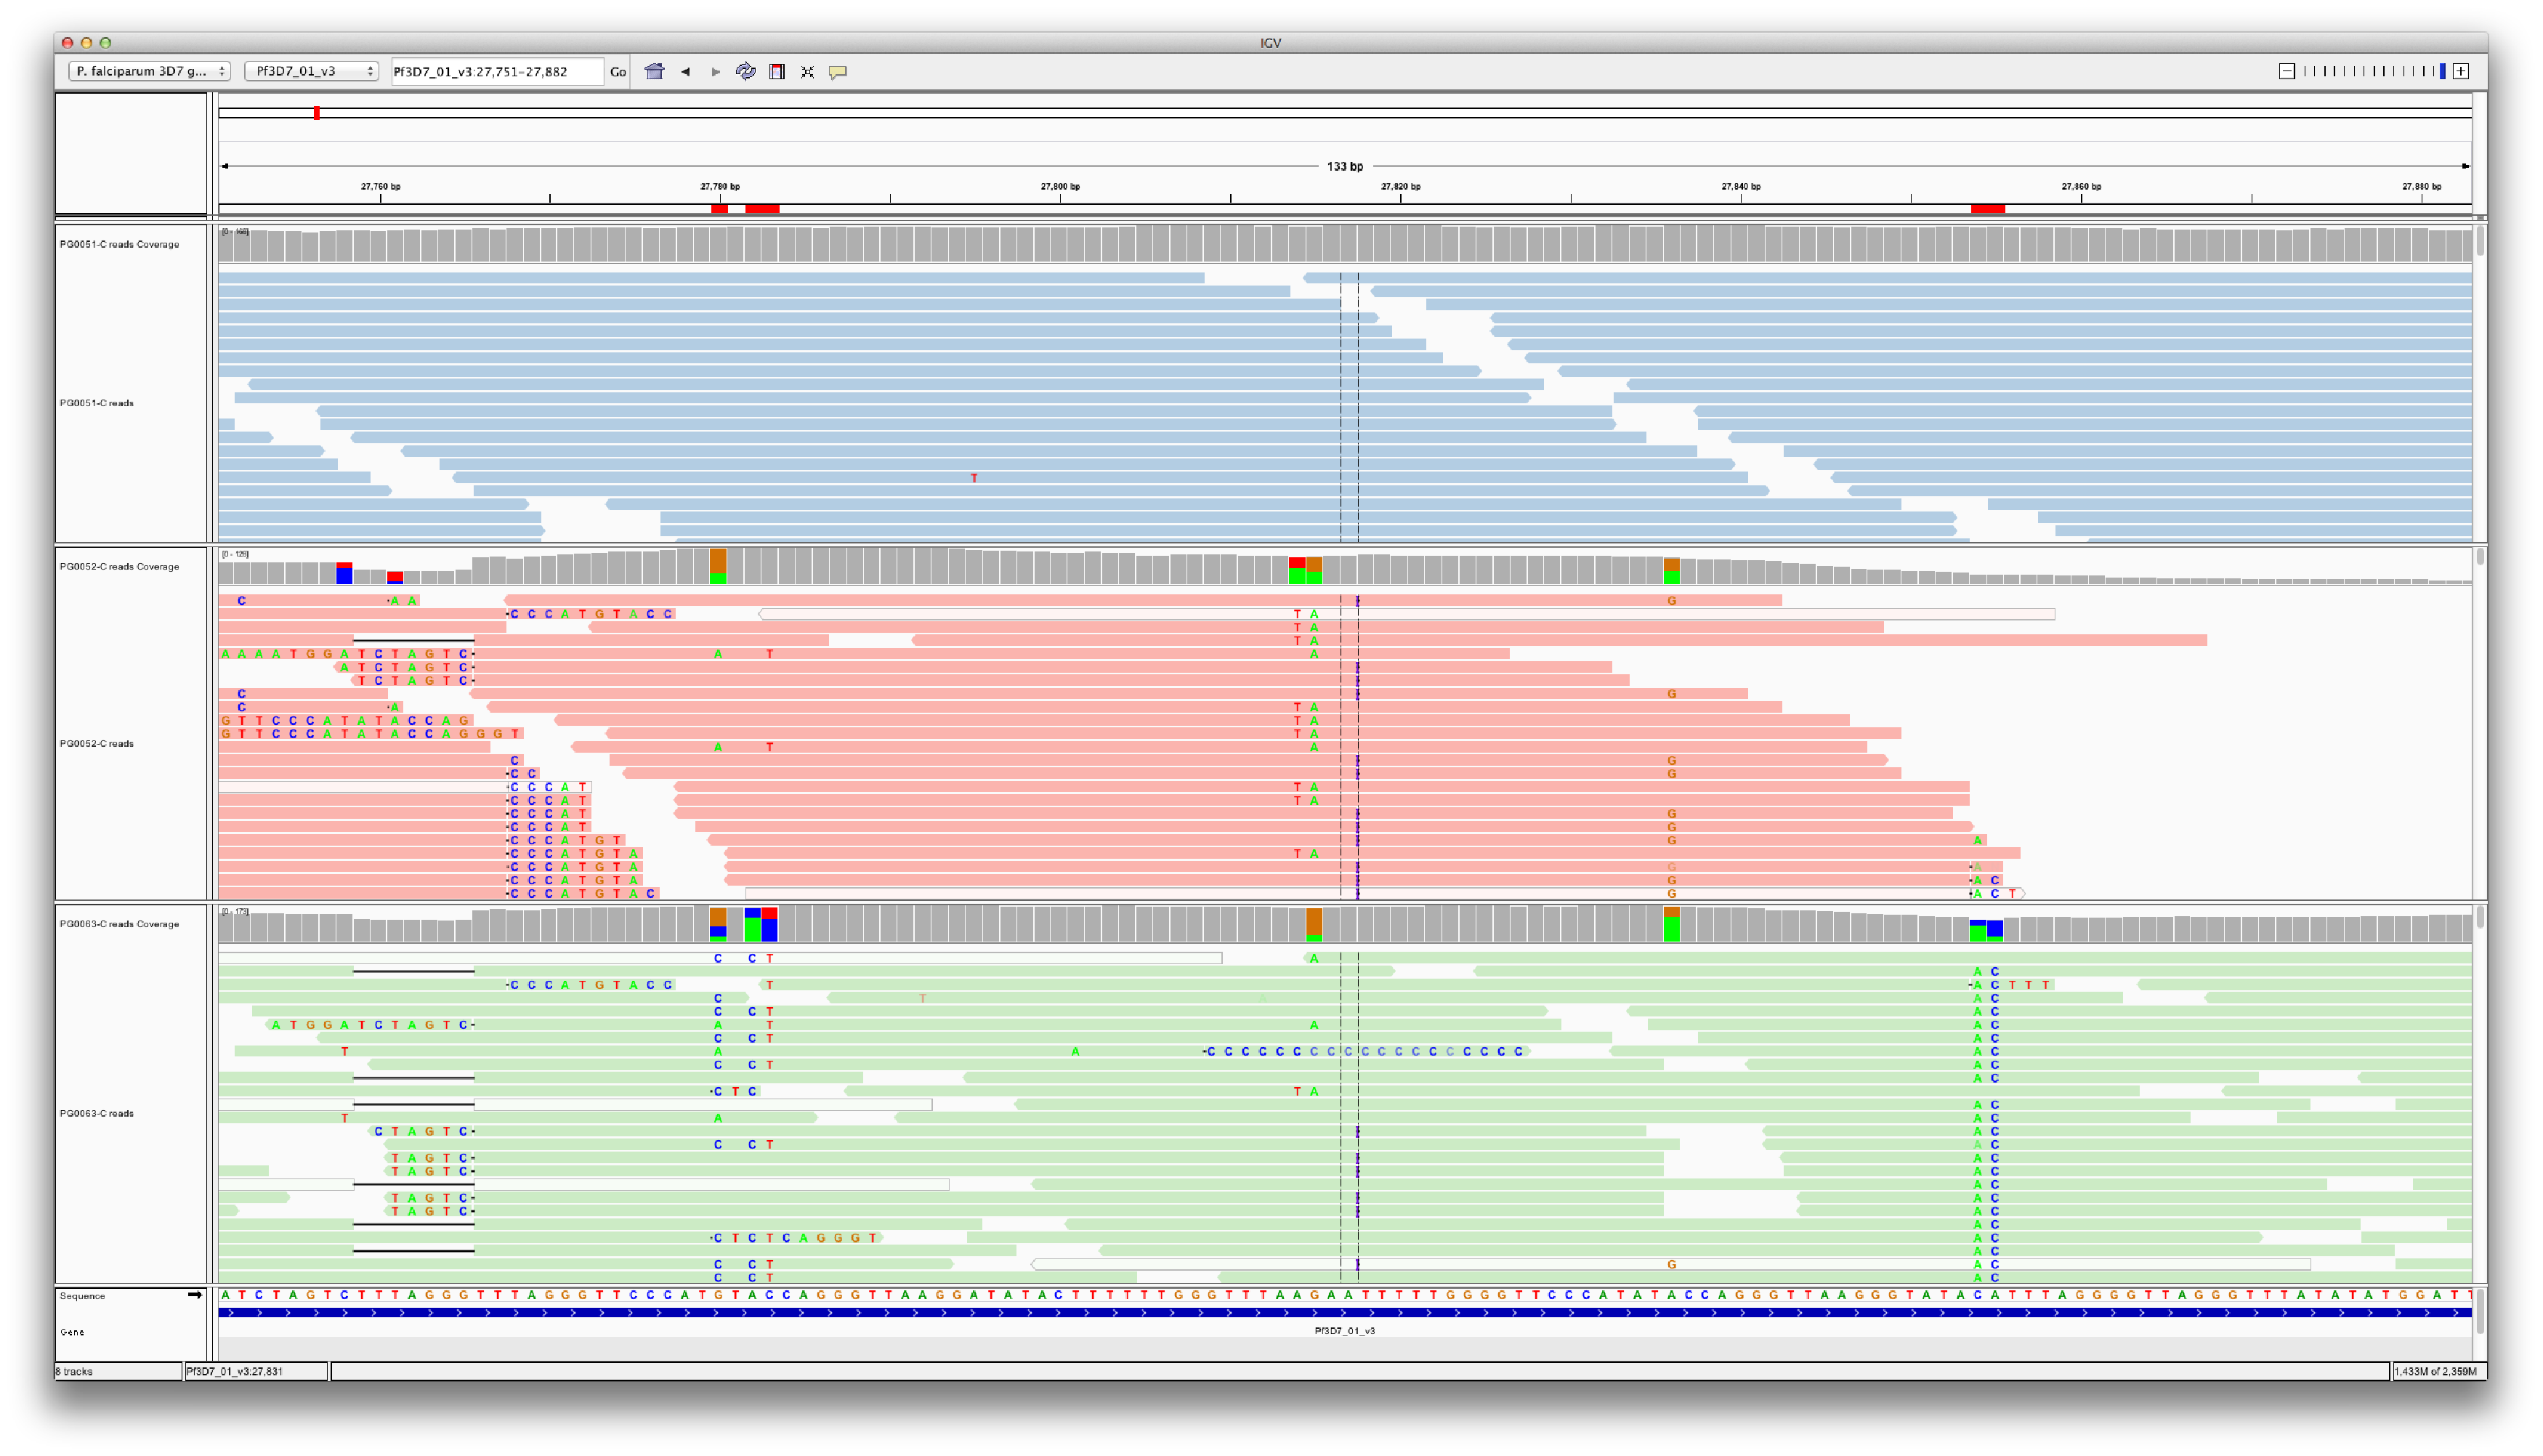
\includegraphics[width=\textwidth]{event1a-c}
  \caption{IGV screenshot of PG0063-C event $1$ (a-c), SNP and two MNPs: three apparent \textit{de novo} mutations within a much larger NAHR event.  Top panel: 3D7 parent.  Middle panel: HB3 parent.  Lower panel: PG0063-C child.  Variant positions are shown as red blocks at the top of the three panels below the genome position track.  Stacked barplots above variant positions indicate the proportion of bases supporting an alternate allele to the reference.}
  \label{fig:event1a-c}
\end{sidewaysfigure}

\begin{figure}[h!]
  \centering
    \includegraphics[width=\textwidth]{{event1a-c.graph}.pdf}
  \caption{Graph screenshot of event $1$ (a-c), SNP and two MNPs: three apparent \textit{de novo} mutations within a much larger NAHR event shown as two bubbles with novel kmer involvement in the upper and middle-left sections of the plot.}
  \label{fig:event1a-cgraph}
\end{figure}

\begin{sidewaysfigure}[h!]
  \centering
    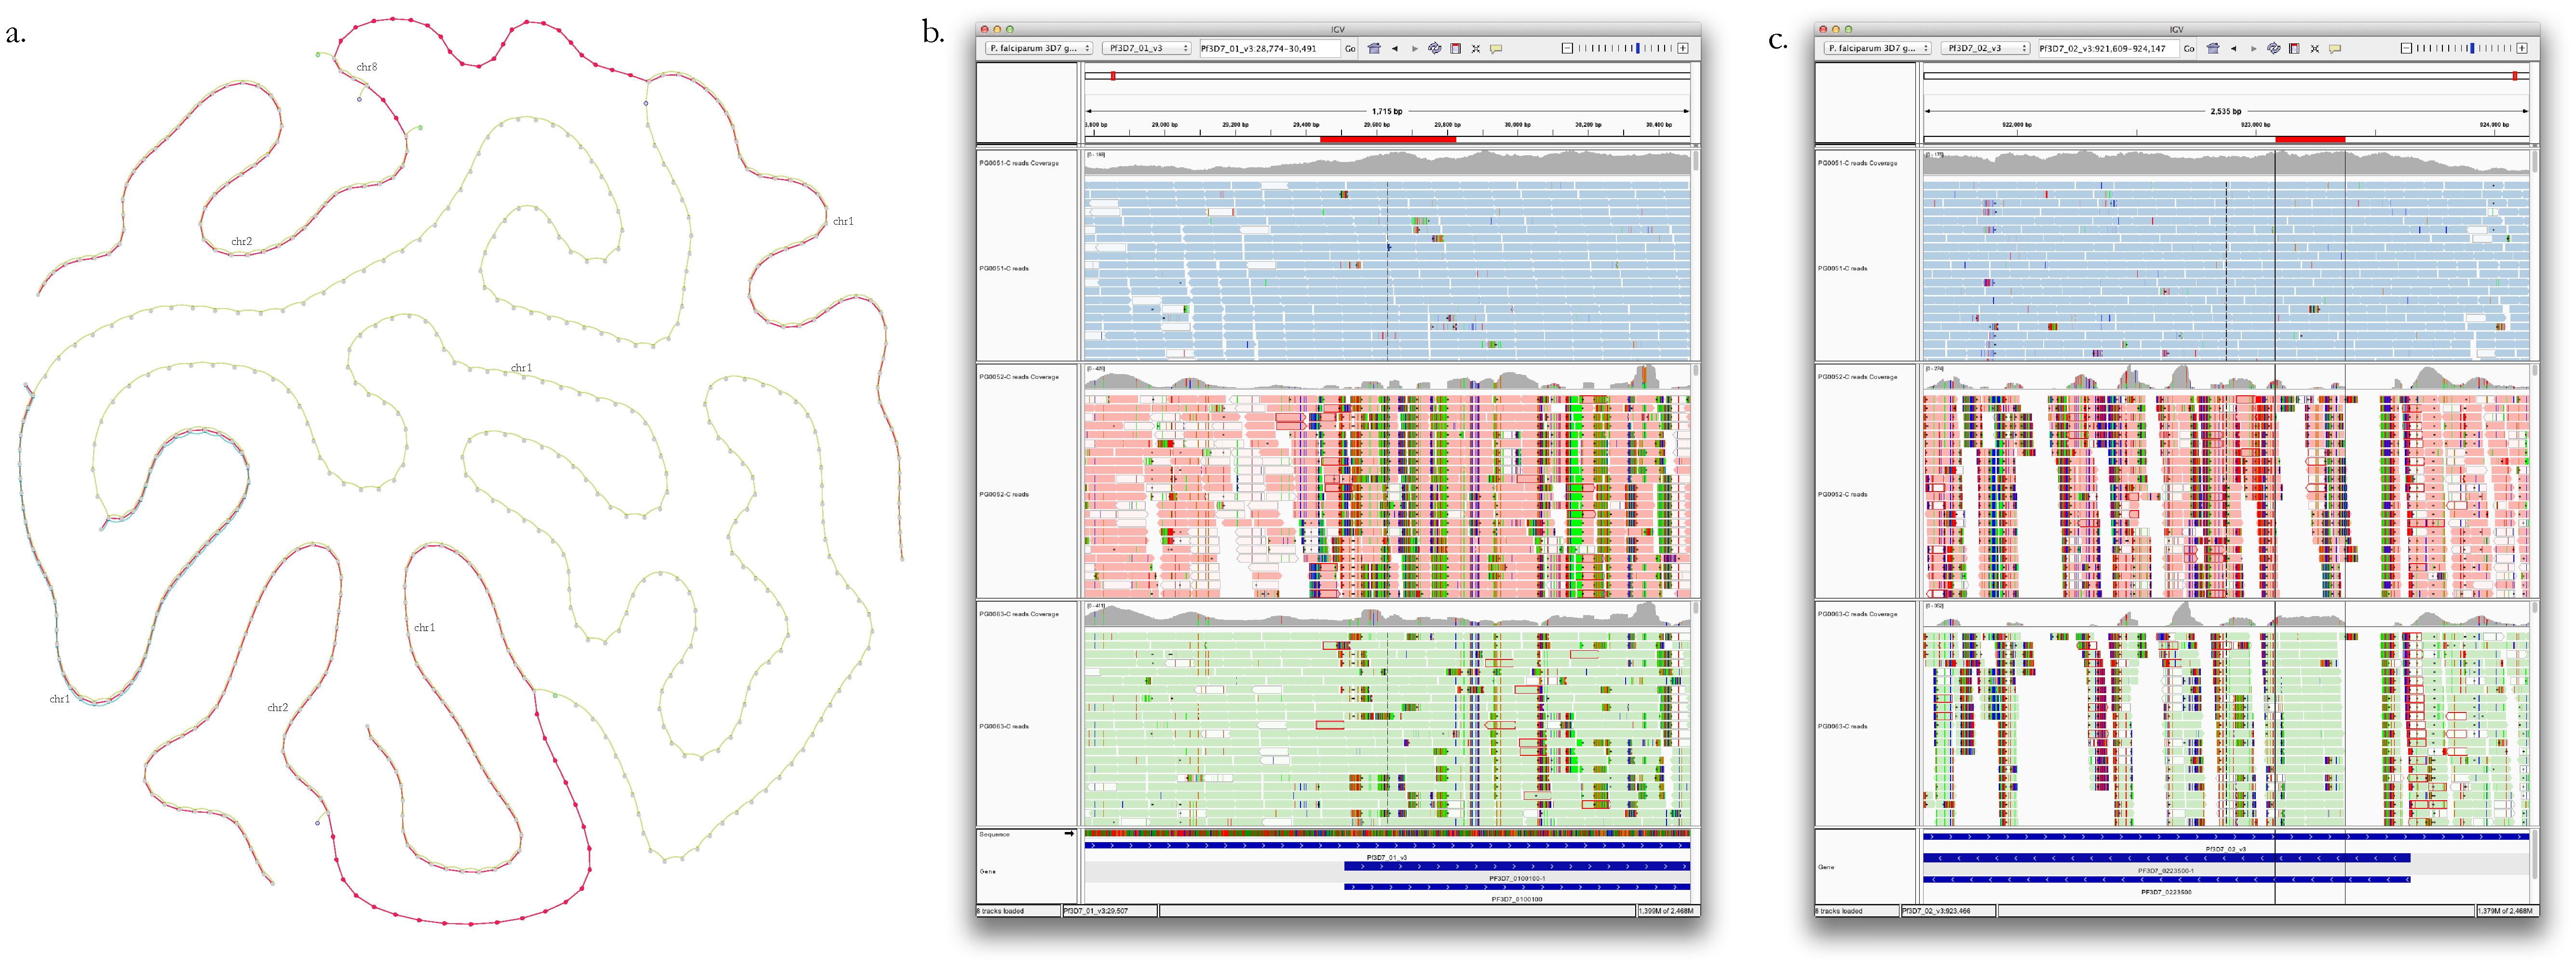
\includegraphics[width=\textwidth]{event1d-h}
  \caption{IGV and graph screenshots of event $1$ (d-h), a NAHR event.  a. Graphical view of the exchange; chromosome of origin specified for various regions.  b. IGV screenshot for 3D7 (top), HB3 (middle), and PG0063-C (child) on the chromosome $1$ region of the event.  c. IGV screenshot of the chromosome $2$ region of the event.}
  \label{fig:event1d-h}
\end{sidewaysfigure}

\begin{sidewaysfigure}[h!]
  \centering
    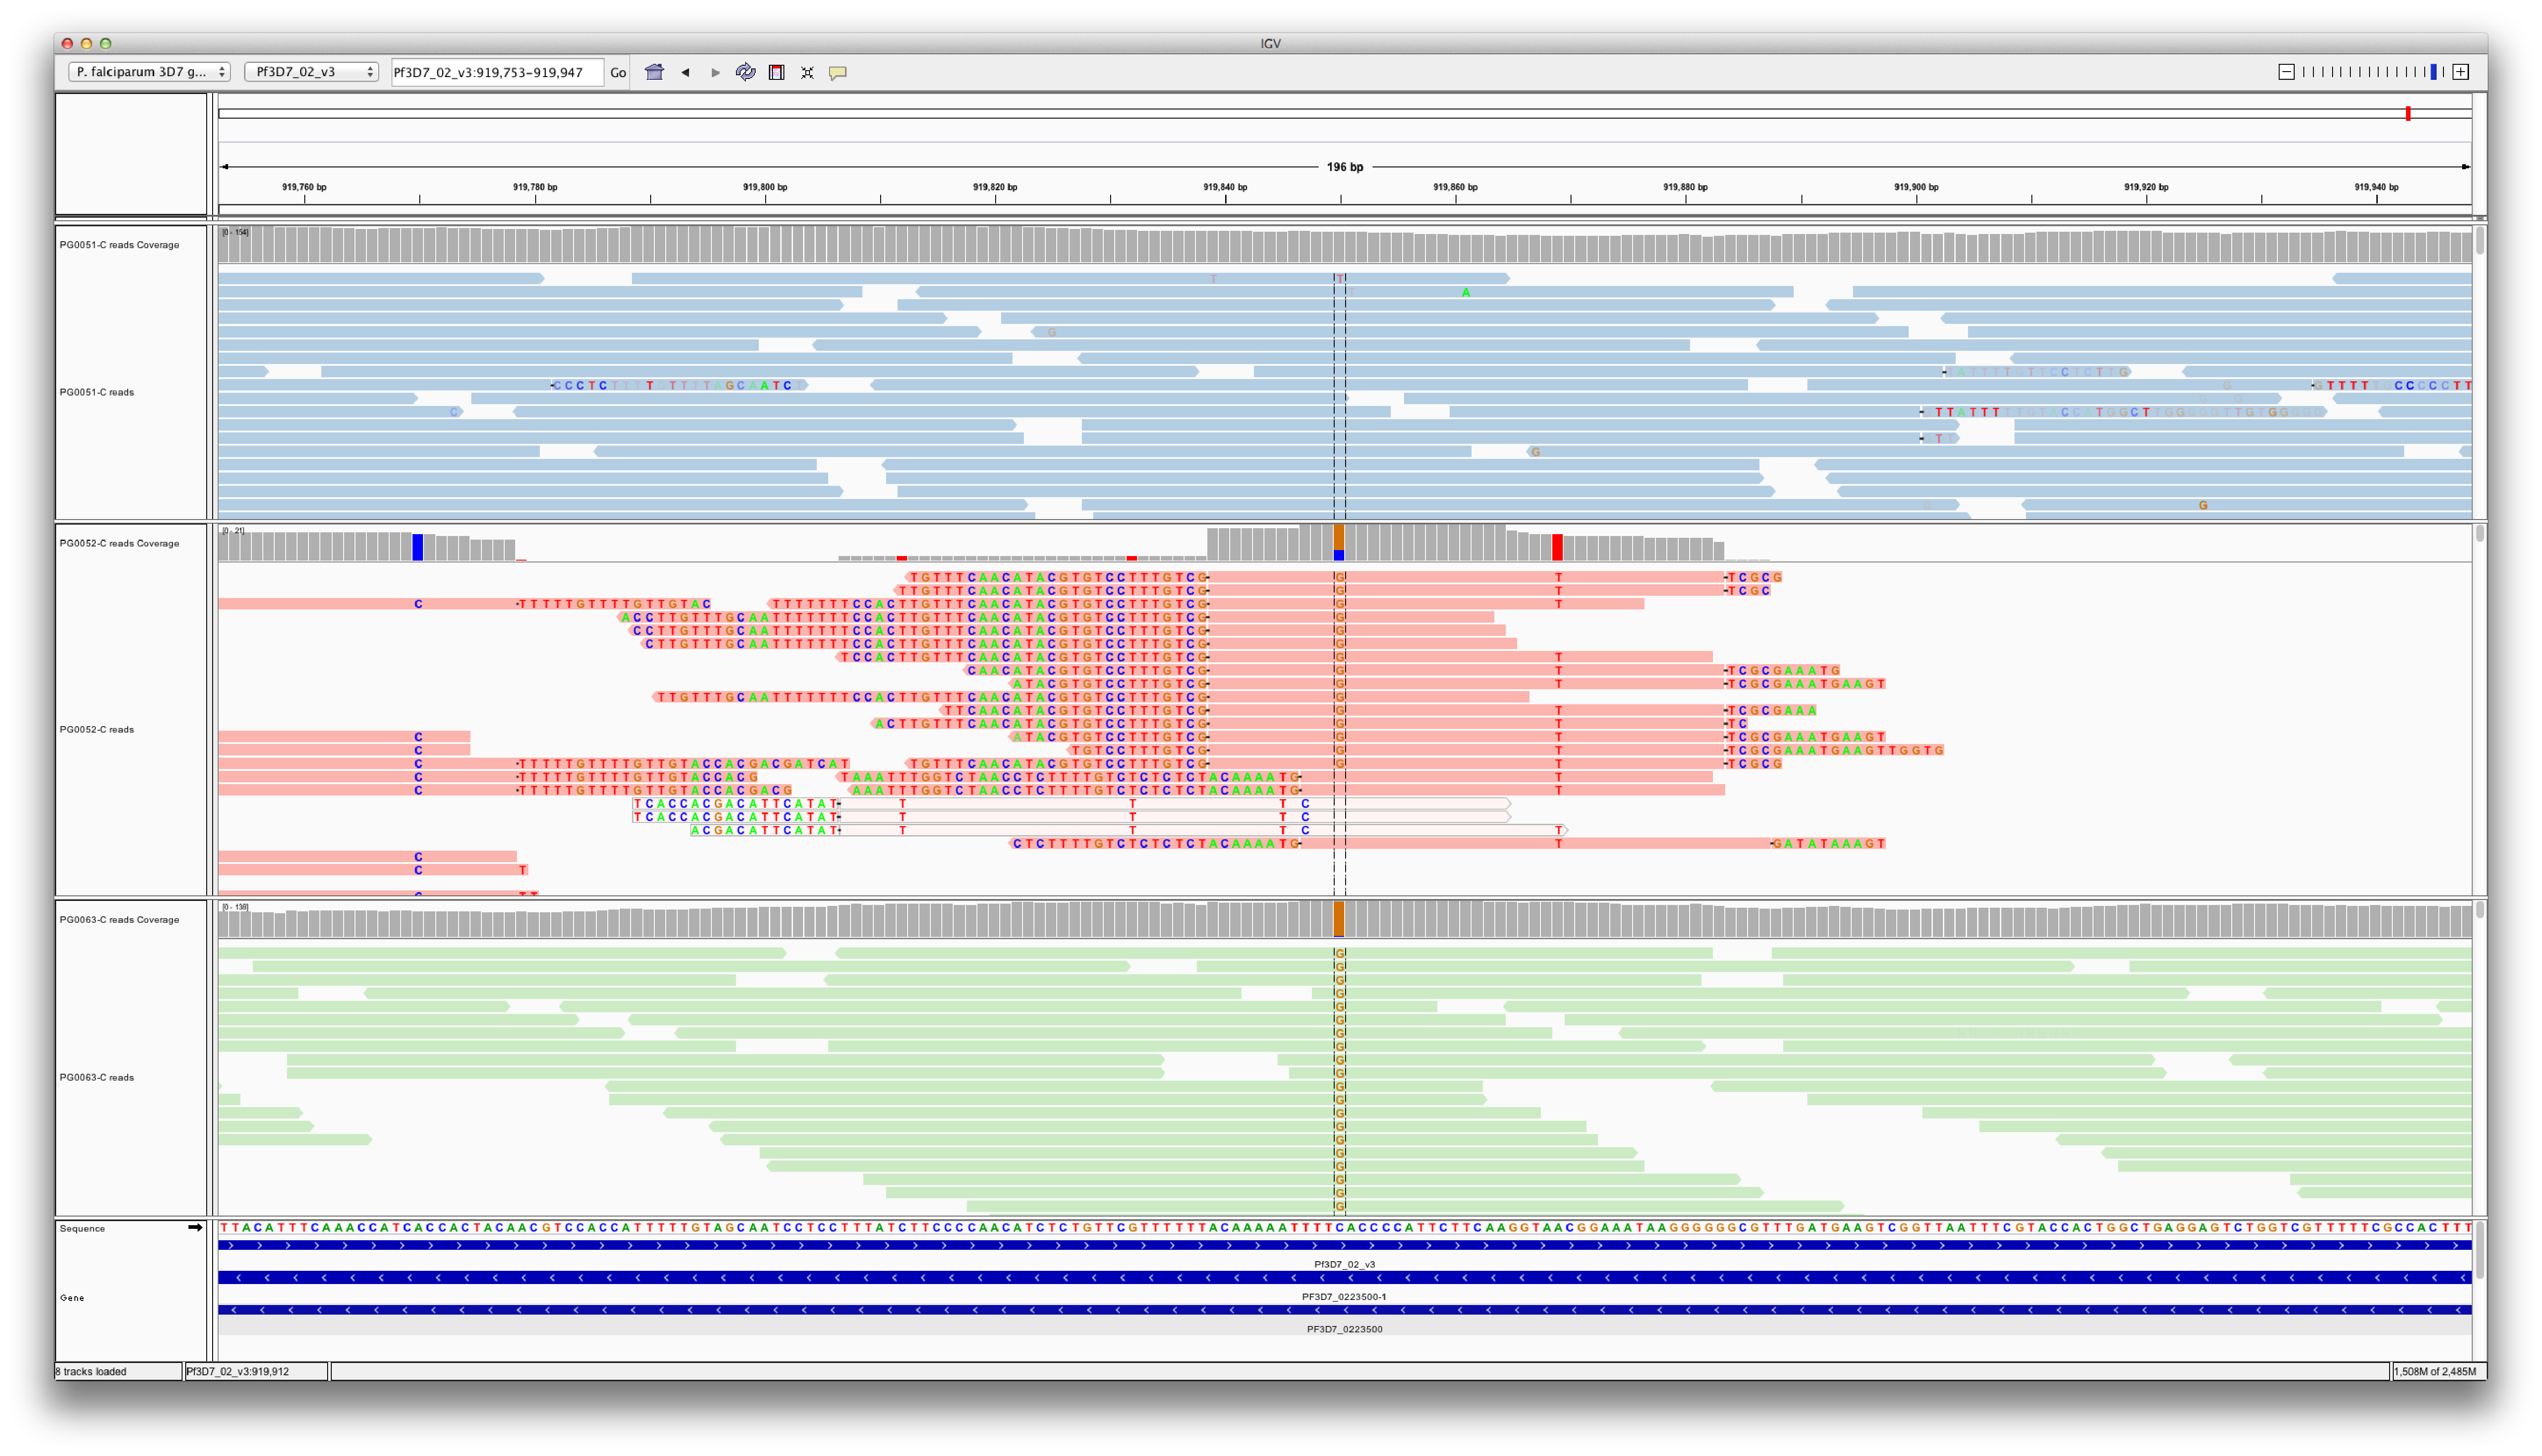
\includegraphics[width=\textwidth]{funnysnp}
  \caption{Event $1$ h: a \textit{de novo} SNP in a \textit{var} on the 3D7 haplotypic background.  Top panel: 3D7.  Middle: HB3.  Lower: PG0063-C child.}
  \label{fig:funnysnp}
\end{sidewaysfigure}

\begin{figure}[h!]
  \centering
    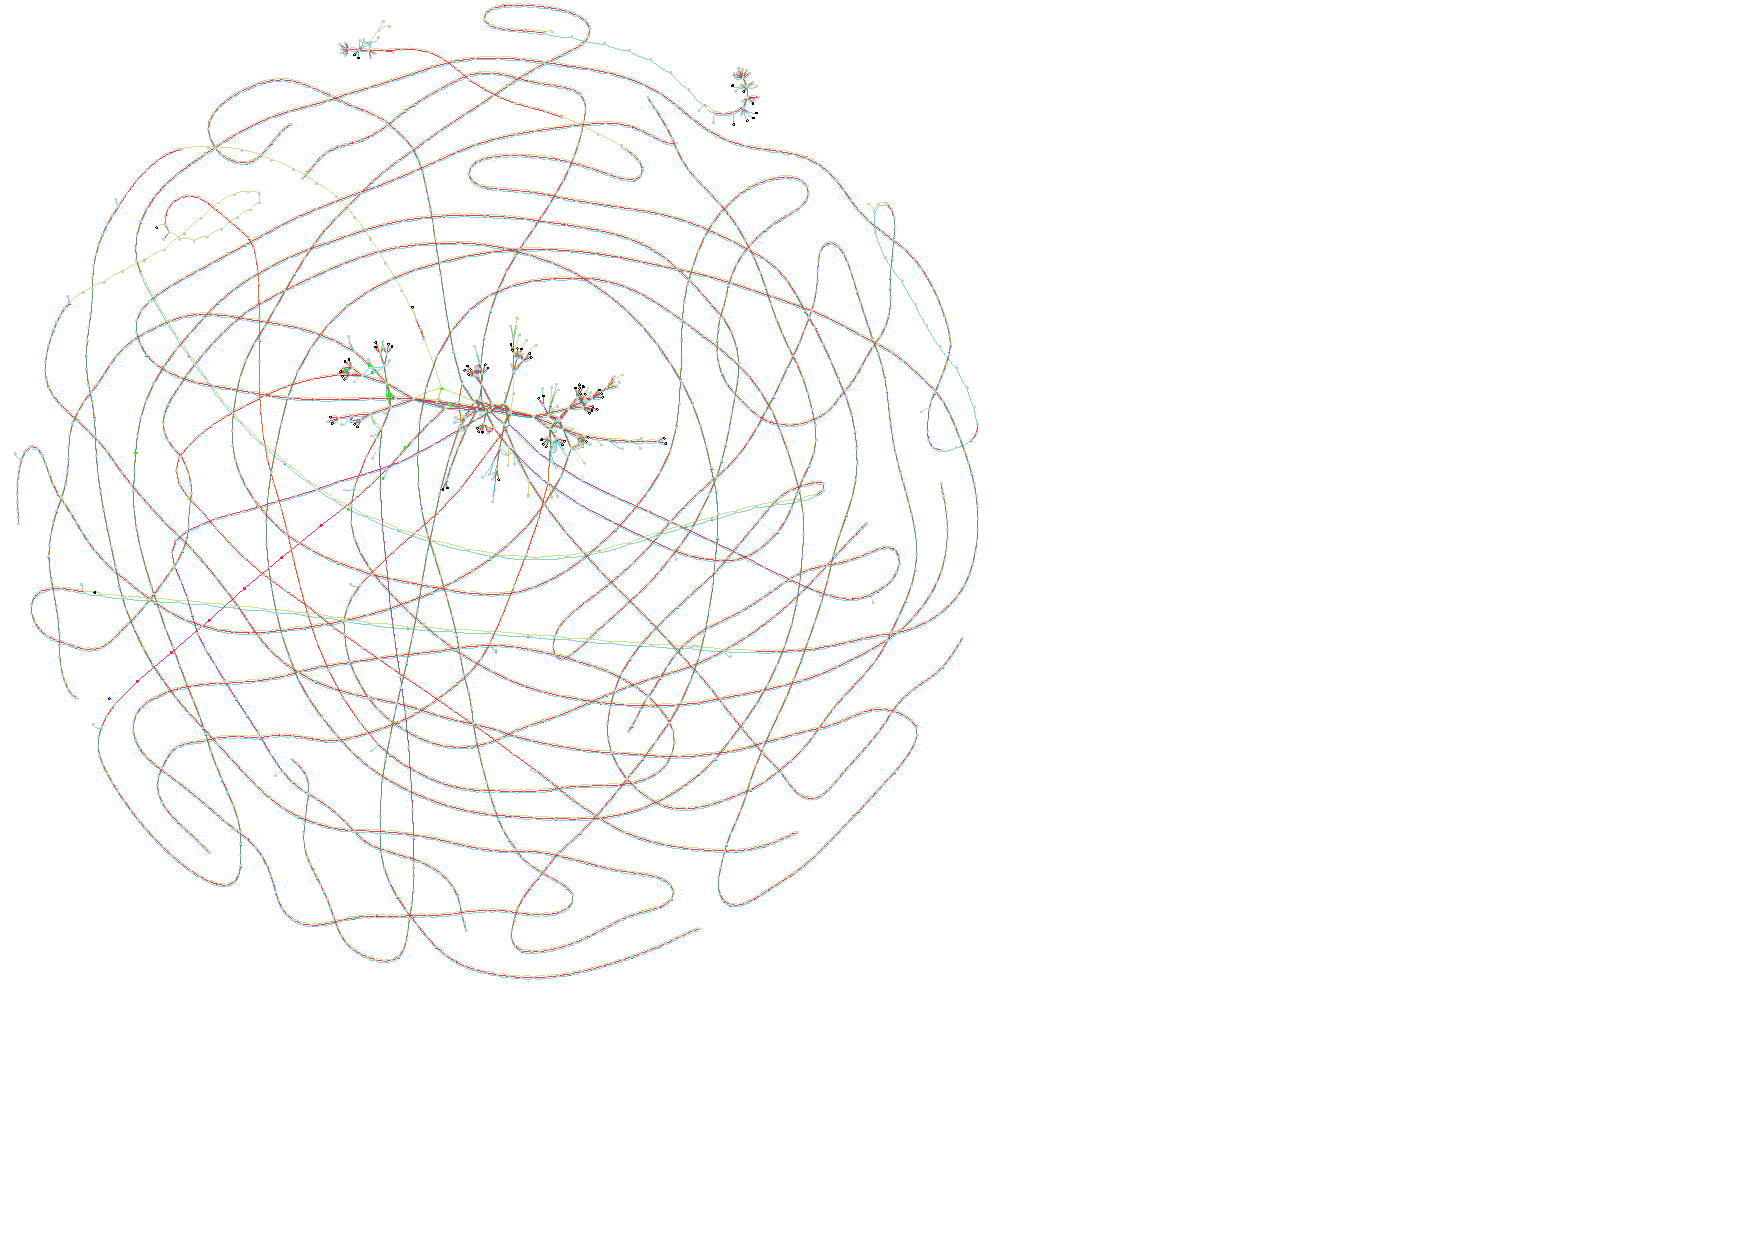
\includegraphics[width=\textwidth]{tangle}
  \caption{Event $2$, a graph "tangle": a region of the graph where the in/out degree of vertices within a small radius sharply increases, resulting from attempting to traverse a low-complexity region of the genome.}
  \label{fig:tangle}
\end{figure}

\begin{sidewaysfigure}[h!]
  \centering
    \includegraphics[width=\textwidth]{{tangle.igv}.pdf}
  \caption{IGV screenshot of event $2$, a low-complexity region of the genome containing many reads with many apparent errors.}
  \label{fig:tangle.igv}
\end{sidewaysfigure}

\begin{sidewaysfigure}[h!]
  \centering
    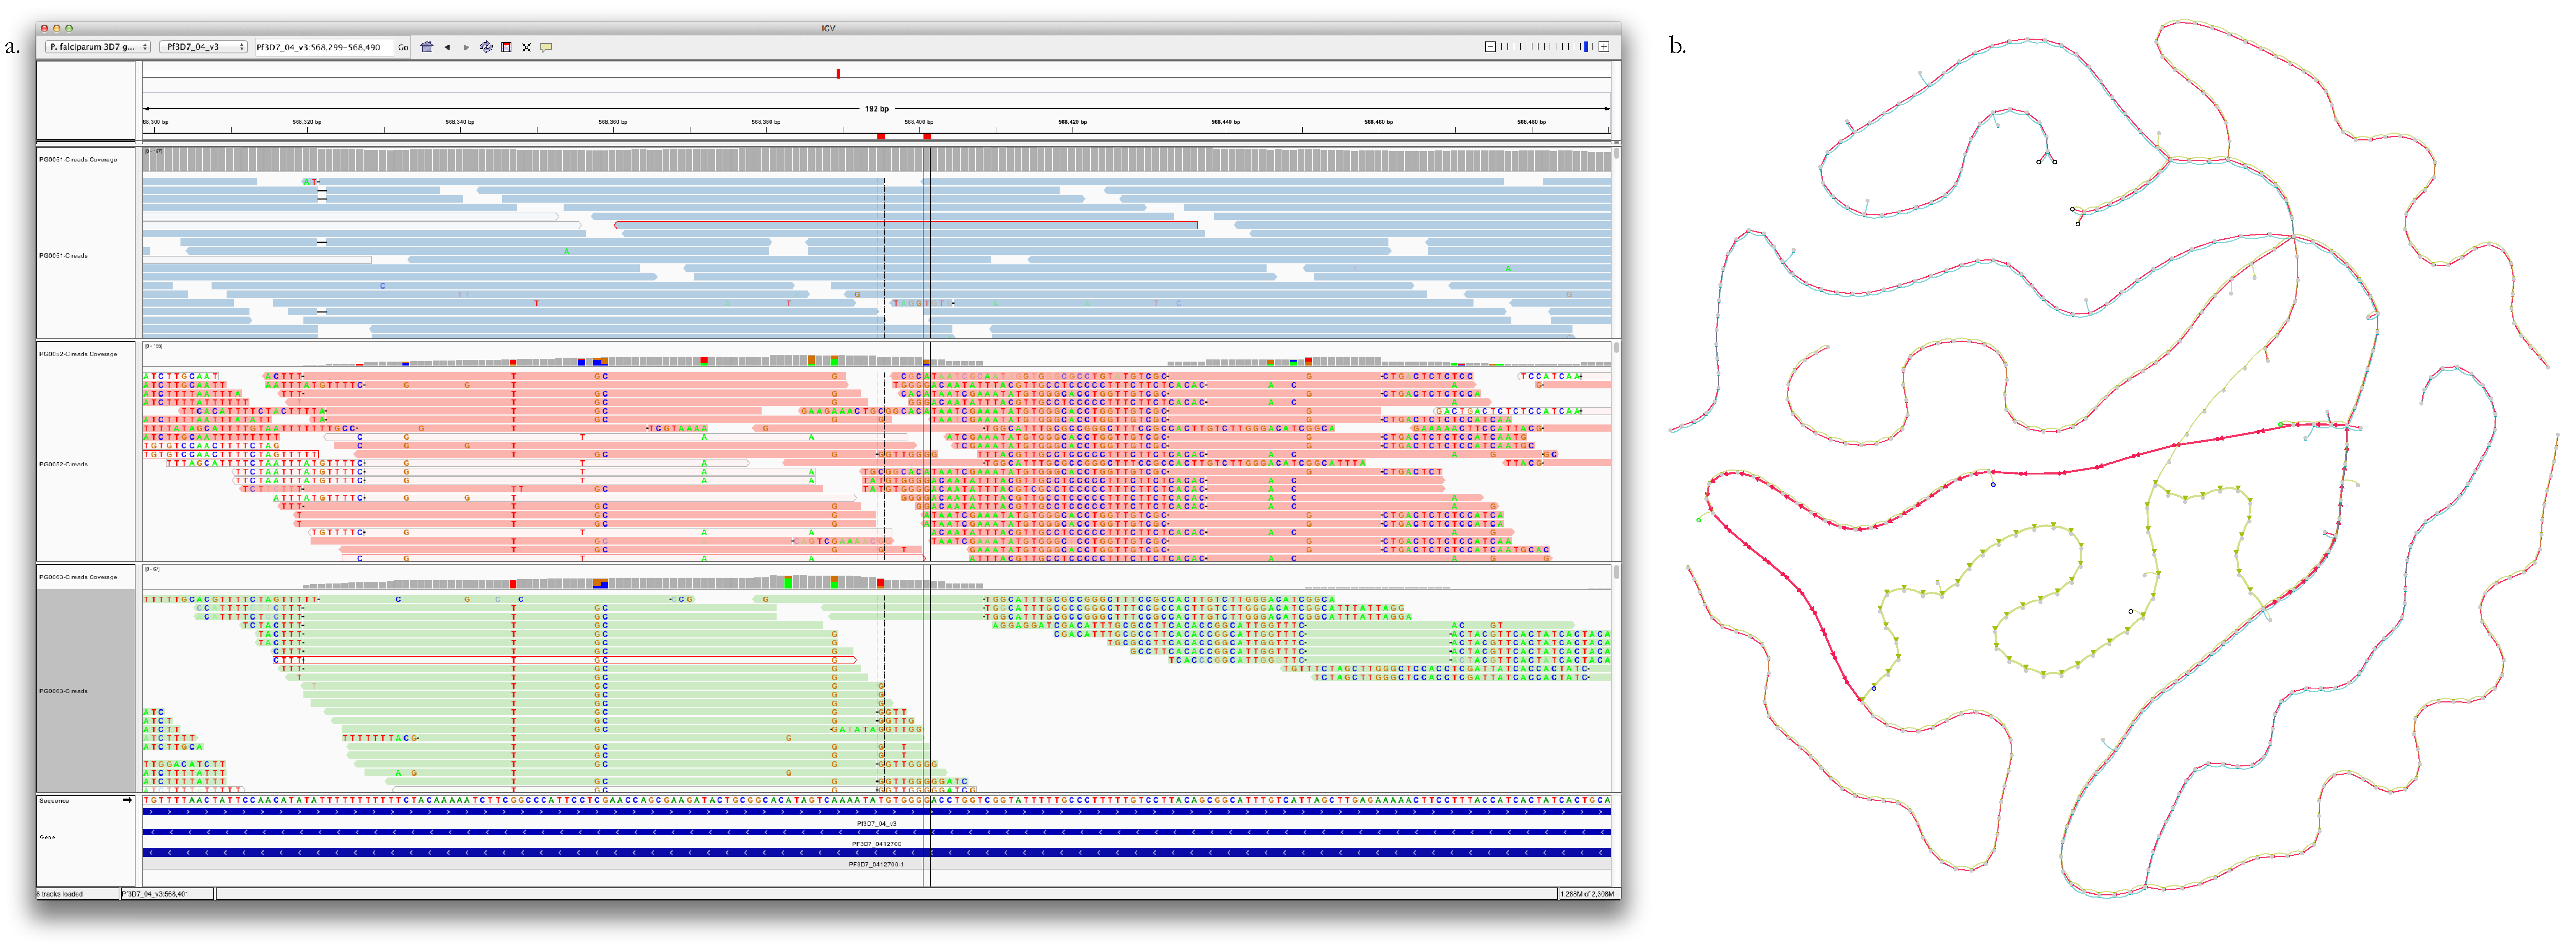
\includegraphics[width=\textwidth]{twosnps}
  \caption{Events $3$ and $4$, two SNPs, non-obvious from the alignments, but apparent in graph.  a. IGV screenshot of two \textit{de novo} SNPs in a \textit{var} gene.  b. Graphical view of the two SNPs.}
  \label{fig:twosnps}
\end{sidewaysfigure}

\begin{sidewaysfigure}[h!]
  \centering
    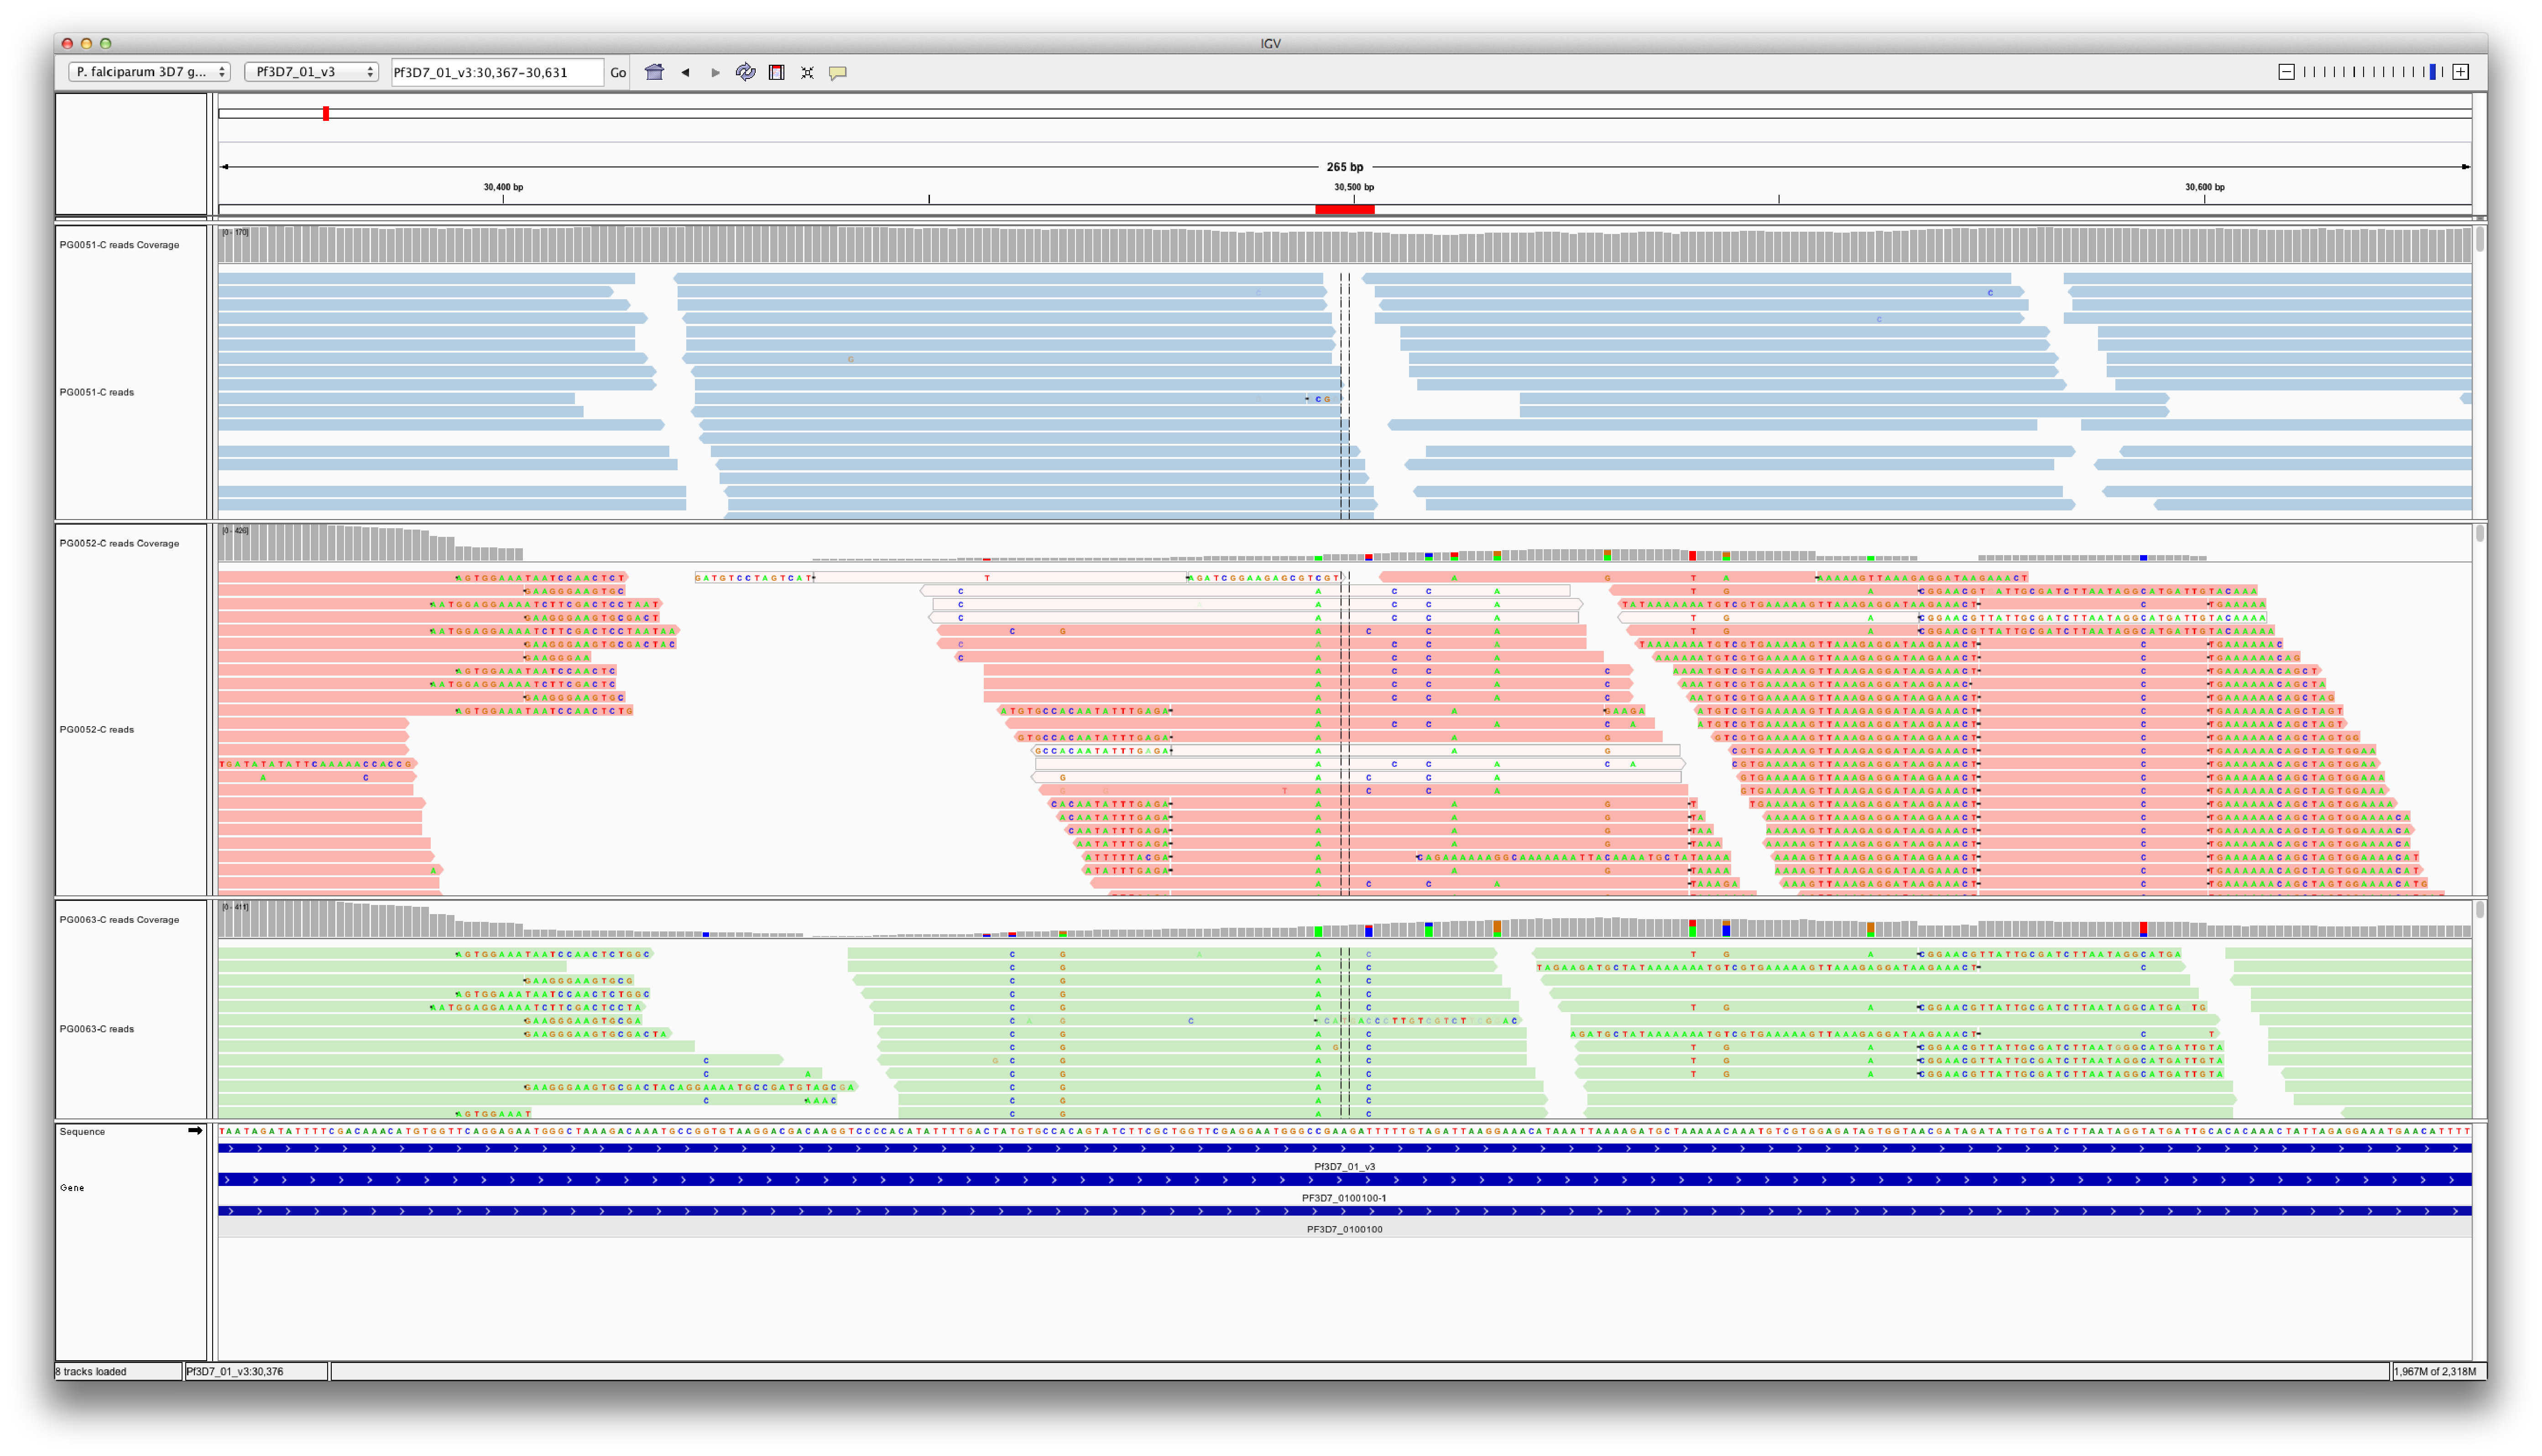
\includegraphics[width=\textwidth]{misplacedsnp}
  \caption{The true home of the events $3$ and $4$, two SNPs misplaced during alignment.}
  \label{fig:misplacedsnp}
\end{sidewaysfigure}
